\documentclass[hidelinks,a4paper, 12pt]{article}
\usepackage[french]{babel}
\usepackage[utf8]{inputenc}
\usepackage[T1]{fontenc}
\usepackage{lmodern}
\usepackage{graphicx}
\usepackage{hyperref}
\usepackage{listings}
\usepackage{color}
\usepackage[titletoc,title]{appendix}
\lstset{language=C,rangeprefix=//---------------,rangesuffix=----------------,includerangemarker=false,columns=spaceflexible,extendedchars=true,showspaces=false,showstringspaces=false,inputencoding=ansinew,tabsize=4,frame=shadowbox,morecomment=[is]{\#ifdef}{\#endif},morecomment=[is]{/*}{*/}}
\title{Lecture et rédaction scientifiques: \\Skip-lists }
\author{Steve Zaretti}

\begin{document}
	
	\maketitle
	\newpage
	\tableofcontents
	\newpage
	
	\section{Introduction}
	\subsection{Liste chainée}
	Une liste chainée est une structure de données de taille arbitraire. Le principe est que chacun des éléments de cette liste contient une référence vers l'élément suivant. Cette pratique facilite l'insertion et la suppression des éléments, au détriment de la rapidité de la recherche.
	
	\subsubsection*{Les alternatives}
	Il existe de nombreuses alternatives aux listes chainées pour trouver un élément plus rapidement: les tables de hashages, les arbres binaires, etc. Mais certaines séquences d'insertions peuvent être catastrophiques. Par exemple, insérer des éléments croissants dans un arbre binaire provoque un rééquilibrage de l'arbre. En revanche, si les éléments sont insérés de façon aléatoire, l'équilibrage devient plus rare.

	Grâce aux probabilités, les \og skip-list \fg{} bénéficient d'un atout majeur: aucune séquence ne peut provoquer systématiquement le pire scénario. Mieux encore, les skip-lists utilisent des algorithmes plus simples et rapides que ses concurrents. Les skip-lists sont aussi très légères et peuvent être configurées pour n'utiliser que $1\frac{1}{3}$ pointeurs par élément.
	
	%% TODO: Insérer illustration
	
	\newpage
	\subsection{Skip-List}
	 Une skip-list bénéficie des avantages de la liste chainée, sans ses inconvénients. Cette structure de données utilise les chaines de façon parallèle. Une fonction basée sur des probabilités permet de déterminer si une nouvelle chaine doit être utilisée ou non. Cette couche supérieure est un moyen plus rapide d'accéder à cet élément.
	\begin{center}
		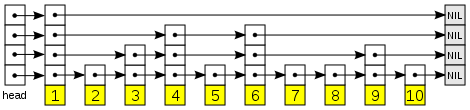
\includegraphics[width=\textwidth]{img/SkipList}
	\end{center}
	\subsubsection*{Définition}
	\begin{itemize}
		\item La hauteur maximale d'une skip-list est définie lors de sa création. Bien qu'il n'y ait pas de taille maximale d'une skip-list, il est conseillé d'utiliser $log_2(n)$ où $n$ est le nombre d'éléments théoriques présents dans la liste. 
		\item Le niveau le plus bas de la liste mène au nœud suivant. %% TODO: Cette phrase est floue, à reformuler.
		\item Les nœuds supérieurs pointent vers un nœud plus avancé dans la liste.  Une couche supérieure est une voie rapide vers la couche inférieure. Ainsi, la couche la plus haute contient les plus grands sauts.
		\item Le parcours d'une skip-list se fait de haut en bas, et de droite à gauche. Si la clé de l'élément suivant sur une couche est plus grande que celle qu'on recherche, celle-ci continue sur une voie inférieure.
		\item L'insertion dans la liste utilise une fonction de probabilité afin de définir sa hauteur maximale.
	\end{itemize}
	
	\newpage
	\section{Les algorithmes}
	Une skip-list a besoin d'avoir un pointeur vers sa tête $(node* head)$. La liste doit connaitre le nombre de voies actuellement utilisé $(size)$. Selon les implémentations, il est possible de définir un nombre de voies maximal $(levelMAX)$. Il est aussi possible de changer le paramètre $(p)$ de probabilité de création d'une nouvelle voie. La variation de ses deux derniers paramètres est étudiée dans le chapitre \nameref{perf}.
	\lstinputlisting[linerange=BEGINSKStruct-ENDSKStruct]{SkipList/SkipList.h}
	
	L'initiation se fait de la manière suivante:
	\begin{itemize}
		\item La hauteur maximale est déterminée par le nombre d'éléments totaux $(n)$ présent dans la liste. Pour des questions de rapidité, la valeur $log_2(n)$ est recommandée.
		\item Création d'un élément $NIL$ possédant une clé plus grande que le maximum autorisé.
		\item Définitions dès ses pointeurs $forward$ vers lui-même.
		\item Le nombre de voies actuelles est fixé à 1.
		\item Le pointeur de tête est défini par cet élément $NIL$.
	\end{itemize}
	\emph{L'algorithme écrit en langage C figure en annexe \ref{SKInit}.}
	
	%% TODO: Insérer illustration
	
	\subsection{La recherche}
	La recherche d'un élément s'exécute de la façon suivante:
	\begin{enumerate}
		\item Commencer l'exploration de la liste par l'élément en tête, et se positionner sur la plus haute voie.
		\item Sur la voie actuelle, regarder la clé de l'élément suivant.
		\item S'elle est plus grande et qu'il existe une voie inférieure, descendre d'une voie.
		\item Sinon aller en 2.
		\item Si la clé de l'élément suivant correspond à celle qui est recherchée: l'élément a été trouvé.
		\item Sinon, l'élément n'a pas été trouvé.
	\end{enumerate}
	\emph{L'algorithme écrit en langage C figure en annexe \ref{SKSearch}.}
	%% TODO: Insérer illustration
	
	\subsection{La hauteur}
	La notion de hauteur est très importante dans une skip-liste. En effet, celle-ci permet de définir à combien de nœuds un élément est attaché. Si trop d'éléments possèdent la même hauteur, la recherche devient trop lente.	Cette méthode est définie à l'aide d'une fonction aléatoire. La hauteur ne dépend ni de la clé de l'élément ni de sa valeur. La fonction aléatoire doit être définie pour qu'un élément de hauteur $h$ possède le double de probabilité qu'un élément de hauteur $h+1$. Ainsi, si un nœud de hauteur 1 a une probabilité $p$ de $0.5$ alors le niveau 2 a une probabilité de $0.25$.
	%% TODO: Insérer illustration
	
	\subsection{L'insertion}
	L'insertion d'un élément dans une skip-liste s'effectue de la façon suivante:
	\begin{enumerate}
		\item Commencer l'exploration de la liste par l'élément en tête, et se positionner sur la plus haute voie.
		\item Sur la voie actuelle, regarder la clé de l'élément suivant.
		\item Si elle est plus grande et qu'il existe une voie inférieure, marquer ce nœud. Puis, descendre d'une voie.
		\item Sinon aller en 2.
		\item Si la clé de l'élément suivant correspond à celle qui est recherchée: modifier la valeur de l'élément par celle de la valeur à insérer. \textbf{FIN}.
		\item Sinon, appeler la fonction de probabilité pour récupérer sa valeur $n$.
		\item Si $n$ est plus grand que la hauteur $h$ de la liste, mettre à jour les pointeurs supérieurs à $h$ vers $NIL$. Ensuite, définir la hauteur maximum actuelle $h$ à $n$.
		\item Créer le nœud $x$ de hauteur $n$.
		\item Pour chaque voie de $1$ à $n$.
		\item Mettre à jour les pointeurs de $x$ vers l'élément suivant de l'élément marqué de cette voie.
		\item Mettre à jour les pointeurs de l'élément marqué de cette voie vers $x$.
		\item \textbf{FIN}.
	\end{enumerate}
	\emph{L'algorithme écrit en langage C est présenté en annexe \ref{SKInsert}.}
	%% TODO: Insérer illustration
	
	
	\subsection{La suppression}
	La suppression d'un élément dans une skip-liste s'effectue de la façon suivante:
	\begin{enumerate}
		\item Commencer l'exploration de la liste par l'élément en tête, et se positionner sur la plus haute voie.
		\item Sur la voie actuelle, regarder la clé de l'élément suivant.
		\item Si elle est plus grande et qu'il existe une voie inférieure, marquer ce nœud. Puis, descendre d'une voie.
		\item Sinon aller en 2.
		\item Si la clé de l'élément suivant ne correspond pas à celle qui est recherchée, \textbf{FIN}.
		\item Sinon pour chaque niveau de l'élément trouvé $x$, mettre à jour les pointeurs de l'élément marqué de cette voie vers l'élément suivant de $x$.
		\item Supprimer $x$.
		\item Si l'élément de tête de la hauteur actuelle de la liste pointe vers $NIL$, diminuer la hauteur actuelle de la liste de 1.
		\item Sinon, \textbf{FIN}.
		\item Si la hauteur est plus grande que 1, aller en 8.
	\end{enumerate}
	\emph{L'algorithme écrit en langage C figure en annexe \ref{SKDelete}.}
	%% TODO: Insérer illustration
	
	\section{Analyse des performances}\label{perf}
	\section{Comparaison avec d'autres structures de données}
	
	
	\begin{appendices}
	\newpage
	\section{Représentation d'une Skip-List en langage C}
	\subsection{Initiation}\label{SKInit}
	\lstinputlisting[linerange=BEGINSKInit-ENDSKInit]{SkipList/SkipList.c}
	\subsection{Fonction aléatoire}\label{SKRandom}
	\lstinputlisting[linerange=BEGINSKRandom-ENDSKRandom]{SkipList/SkipList.c}

	\subsection{Recherche}\label{SKSearch}
	\lstinputlisting[linerange=BEGINSKSearch-ENDSKSearch]{SkipList/SkipList.c}

	\subsection{Insertion}\label{SKInsert}
	\lstinputlisting[linerange=BEGINSKInsert-ENDSKInsert]{SkipList/SkipList.c}
	
	\subsection{Suppression}\label{SKDelete}
	\lstinputlisting[linerange=BEGINSKDelete-ENDSKDelete]{SkipList/SkipList.c}
	\newpage
	\end{appendices}
	
	
	@online{1,
		author = {Patrice Roy},
		title = {Skip Lists},
		date = {27/02/2016},
		url = {http://h-deb.clg.qc.ca/Sujets/Structures-donnees/SkipLists.html},
	}
	@online{2,
		author = {Sylvie Hamel},
		title = {Dictionnaires ordonnés et “Skip List”},
		date = {25/02/2016},
		url = {http://www.iro.umontreal.ca/~hamelsyl/SkipList.pdf},
	}
	
\end{document} 